\section{Проверка соответствия реализации и спецификации}

После построения TLA+-спецификации алгоритма Raft следующим шагом стала
проверка того, насколько фактическое поведение реализации совпадает с
поведением, допускаемым формальной моделью. В данной работе использовался не
подход ``доказать корректность исходного кода напрямую'', а более практичная и
воспроизводимая схема валидации трасс исполнения: программа
инструментировалась таким образом, чтобы во время работы порождать
машиночитаемую трассу абстрактных событий, после чего эта трасса проверялась
модельным проверяющим TLC на соответствие спецификации \texttt{Raft.tla} (см.
Приложение Б).

Такой подход оказался особенно полезен по двум причинам. Во-первых, он
позволяет проверять не отдельные локальные свойства кода, а целостные сценарии
исполнения распределённой системы, включая выборы лидера, обмен RPC-сообщениями
и переходы между ролями узлов. Во-вторых, он даёт строгий критерий
несоответствия: если TLC не может сопоставить очередной шаг трассы с допустимым
действием спецификации, значит либо реализация действительно ведёт себя не так,
как предписывает модель, либо ошибка содержится в инструментировании или
вспомогательной обвязке проверки. Поэтому существенная часть работы заключалась
не только в запуске TLC, но и в аккуратной организации всей цепочки
``реализация~$\rightarrow$~трасса~$\rightarrow$~абстрактная модель''.

\subsection{Инструментирование реализации}

Для проверки соответствия в реализацию Raft был встроен отдельный механизм
трассировки, задача которого состояла не в обычном логировании отладочных
сообщений, а в фиксации именно тех изменений, которые имеют смысл с точки
зрения спецификации. Иными словами, трассировщик должен был отражать не
внутренние детали реализации, а переходы абстрактной модели: отправку и
получение сообщений, изменение терма, переходы между ролями
\texttt{Follower/Candidate/Leader}, учёт голосов, обновление индексов
репликации и т.д.

Инструментирование было выполнено на уровне класса
\texttt{RaftConsensus}. В ключевых точках алгоритма были добавлены вызовы
специального объекта \texttt{RaftTracer}. Этот объект формировал записи трассы
в формате NDJSON, по одной JSON-строке на событие. Каждая запись содержала:

\begin{itemize}
    \item имя абстрактного события, например \texttt{RequestVote},
    \texttt{BecomeLeader}, \texttt{AppendEntries},
    \texttt{HandleRequestVoteRequest},
    \texttt{HandleAppendEntriesResponse},
    \texttt{AcceptAppendEntriesRequest},
    \texttt{RejectAppendEntriesRequest},
    \texttt{UpdateTerm};
    \item набор элементарных операций над переменными модели:
    \texttt{Update}, \texttt{Add}, \texttt{Clear},
    \texttt{AddElement}, \texttt{AddElementToBag},
    \texttt{RemoveElementFromBag};
    \item идентификатор процесса-источника, используемый только для отладки и
    корреляции событий из разных процессов;
    \item при необходимости --- дополнительные аргументы события
    (\texttt{event\_args}), например идентификатор сервера.
\end{itemize}

Особенно важным оказалось то, что одно действие реализации не всегда
соответствует одному действию TLA+-модели. Например, при получении сообщения с
большим термом реализация сначала должна логически выполнить действие
\texttt{UpdateTerm}, а уже затем --- обработать само сообщение
(\texttt{HandleRequestVoteRequest} или \texttt{AcceptAppendEntriesRequest}).
Именно поэтому трассировщик добавлялся не ``на уровень RPC-обработчика
целиком'', а в конкретные точки изменения абстрактного состояния. Без этого TLC
не смог бы сопоставить трассу с последовательностью допустимых переходов
модели.

Каждый процесс записывал трассу в отдельный файл. При запуске узла путь к
файлу передавался через переменную окружения \texttt{TLAC\_TRACE\_FILE}.
Дополнительно через \texttt{TLAC\_CLOCK\_FILE} передавался путь к общему
файлу логических часов, который использовался для согласованного упорядочивания
событий между несколькими процессами. Это было необходимо потому, что при
параллельной работе узлов простого порядка строк в отдельных файлах
недостаточно: для корректной проверки требуется единая линейная трасса.

\subsection{Инфраструктура запуска и проверки}

Для автоматизации экспериментов был собран отдельный набор инструментов,
образующий полноценный конвейер проверки.

Скрипт \texttt{run\_impl.py} отвечал за запуск кластера. Он читал конфигурацию
запуска, поднимал нужное число узлов, выставлял переменные окружения
трассировки, задавал рабочие каталоги и управлял временем жизни процессов.

Скрипт \texttt{pipeline.py} управлял всей процедурой целиком. Он выполнял
следующие шаги:

\begin{enumerate}
    \item загружал конфигурацию запуска;
    \item выбирал один из кластерных сценариев;
    \item формировал активные конфигурационные файлы для реализации и для TLC;
    \item очищал старые трассы, снимки состояния и файл логических часов;
    \item запускал реализацию через \texttt{run\_impl.py};
    \item после завершения прогона собирал все порождённые трассы;
    \item объединял их в один итоговый NDJSON-файл;
    \item запускал TLC на спецификации \texttt{RaftTrace.tla}.
\end{enumerate}

Объединение трасс выполнял отдельный модуль \texttt{trace\_merger.py}. Он
собирал все фрагменты трасс, сортировал их по метаданным логических часов и
удалял служебную информацию, не участвующую в семантике модели. На выходе
получался единый файл \texttt{trace.ndjson}, который затем подавался на вход
TLC.

Сама проверка строилась не на спецификации \texttt{Raft.tla} напрямую, а через
обёртку \texttt{RaftTrace.tla}. Эта обёртка использовала шаблон
\texttt{TraceSpec.tla} и интерпретировала записи NDJSON как последовательность
наблюдаемых переходов системы. Идея состояла в следующем: TLC стартует из
состояния \texttt{Init} и пытается шаг за шагом сопоставить очередную запись
трассы с каким-либо допустимым действием спецификации. Если такое действие
существует, проверка продолжается. Если нет, TLC останавливается и печатает
первый шаг трассы, который не удаётся встроить в допустимое поведение модели.

Именно это свойство делало инструмент очень удобным для локализации ошибок.
Вместо абстрактного сообщения ``инвариант нарушен'' получался вполне конкретный
ответ: например, ``не удалось сопоставить событие \texttt{RequestVote}'' или
``не удалось сопоставить событие \texttt{UpdateTerm}''. Далее можно было
смотреть на содержимое соответствующей записи NDJSON и сравнивать её с тем,
какие предусловия и эффекты имеет соответствующее действие в
\texttt{Raft.tla}.

\subsection{Стратегия тестирования}

На практике выяснилось, что для надёжной локализации расхождений одного
прогона полного трёхузлового кластера недостаточно. Если сразу запускать
максимально сложный сценарий, трасса быстро разрастается, а точка первого
несоответствия может оказаться следствием более ранней ошибки, замаскированной
дальнейшими переходами. Поэтому проверка велась поэтапно.

Сначала использовались кластеры минимального размера: из одного, двух и трёх
узлов. Для этого конфигурация запуска была переработана так, чтобы один и тот
же набор инструментов мог поднимать разные подмножества узлов:
\texttt{single-raft-0}, \texttt{single-raft-1}, \texttt{single-raft-2},
\texttt{pair-raft-0-1}, \texttt{pair-raft-0-2}, \texttt{pair-raft-1-2} и
\texttt{triple-raft-0-1-2}. Такой подход позволял сначала проверить самые
простые режимы, а затем постепенно увеличивать сложность сценария.

Кроме того, перед тем как считать очередное TLC-несоответствие реальным
дефектом реализации, отдельно проверялась корректность самой инфраструктуры
проверки. В ходе работы было обнаружено несколько проблем именно в обвязке:
например, необходимость записывать ``активные'' конфигурационные файлы не в
формате красиво отформатированного JSON, а строго в виде одной JSON-строки,
иначе модуль \texttt{Json} внутри TLC не мог корректно десериализовать вход; или
необходимость явно учитывать, что трассы одного узла могут записываться в
файлы вида \texttt{raft-0.part000.ndjson}, \texttt{raft-0.part001.ndjson} и
т.д. Лишь после устранения подобных проблем стало возможным уверенно
интерпретировать ошибки TLC как ошибки самой реализации.

\subsection{Обнаруженные несоответствия}

В результате проверки были подтверждены два реальных расхождения реализации со
спецификацией \texttt{Raft.tla}. Оба они воспроизводились на трассах, оба
приводили к остановке TLC на конкретном шаге, и для обоих удалось локализовать
причину непосредственно в исходном коде реализации.

\subsubsection*{Несовпадение начального значения \texttt{currentTerm}}

Первое расхождение было обнаружено уже на самых ранних шагах исполнения, в
момент первого запуска выборов. В спецификации начальные значения серверных
переменных задаются следующим образом: каждый сервер стартует в состоянии
\texttt{Follower}, с пустым журналом, с \texttt{votedFor = Nil} и с
\texttt{currentTerm = 1}. Следовательно, первое действие
\texttt{RequestVote(i)} в модели переводит узел из терма $1$ в терм $2$.

В реализации же поле \texttt{current\_term\_} было инициализировано значением
\texttt{0}. Из-за этого первый запуск выборов переводил узел не в терм $2$, а
в терм $1$. На уровне ``обычной'' отладки это могло показаться безобидной
деталью: все узлы всё равно стартуют синхронно, а относительный порядок термов
как будто сохраняется. Однако для формальной спецификации это существенное
расхождение, потому что стартовое состояние модели фиксировано, и вся дальнейшая
траектория строится относительно него.

Практически ошибка проявлялась так: TLC останавливался уже на первом событии
\texttt{RequestVote}, так как в трассе кандидат переходил в
\texttt{currentTerm = 1}, тогда как спецификация ожидала
\texttt{currentTerm = 2}. Иными словами, первое же наблюдаемое действие
реализации не могло быть встроено в допустимое поведение модели.

Это расхождение важно не только потому, что ``не совпадает цифра''.
Начальный терм --- фундаментальная часть состояния Raft. Если реализация и
спецификация различаются уже в стартовой точке, все последующие сравнения
термов, условия \texttt{UpdateTerm}, выборы лидера и правила обработки RPC
становятся смещёнными. Поэтому данная проблема была устранена в первую очередь:
после приведения начального значения \texttt{current\_term\_} к тому, что
ожидает спецификация, трасса стала проходить дальше, и TLC смог выявить уже
следующее, более содержательное расхождение.

\subsubsection*{Отправка \texttt{RequestVote} самому себе}

Второе подтверждённое несоответствие касалось состава множества peer-ов в
реализации. Согласно спецификации, действие \texttt{RequestVote(i)}
рассылает запросы \texttt{RequestVoteRequest} только серверам из множества
\texttt{Server \textbackslash \{i\}}. Это соответствует стандартной логике
Raft: кандидат учитывает собственный голос локально, через
\texttt{votedFor[i] = i} и \texttt{votesGranted[i] = \{i\}}, и не должен
дополнительно отправлять RPC самому себе (см. рис. \ref{fig:self}.

\begin{figure}[h]
    \centering
    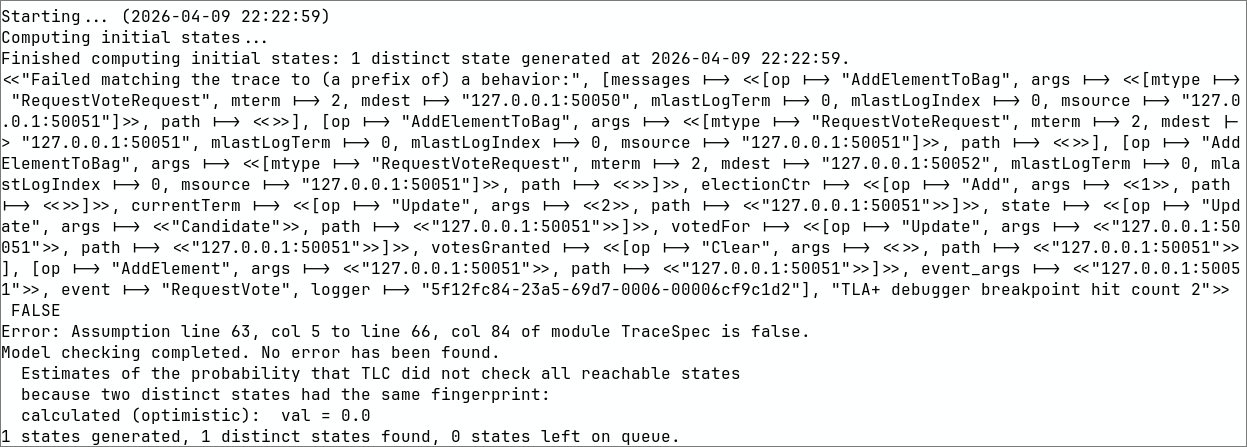
\includegraphics[width=0.82\linewidth]{inc/self_call.png}
    \caption{Нахождение расхождения при отправке запроса самому себе}
    \label{fig:self}
\end{figure}

Однако на трассах реализации было зафиксировано, что узел действительно
порождает сообщение \texttt{RequestVoteRequest}, у которого адрес источника
совпадает с адресом назначения. Это означало, что собственный адрес сервера
ошибочно оставался в пуле peer-соединений, и кандидат начинал отправлять
\texttt{RequestVote} самому себе как обычному соседу.

С точки зрения соответствия спецификации это уже само по себе является
ошибкой: TLA+-модель такого шага не допускает. Но важнее то, что в
реализации это могло искажать саму логику выборов. Собственный голос уже был
учтён локально в момент перехода в состояние кандидата. Если после этого узел
ещё и получал успешный \texttt{RequestVoteResponse} от самого себя, тот же
голос мог быть учтён повторно --- теперь уже как голос от peer-а. В предельном
случае это позволяло кандидату достигнуть ``кворума'' раньше, чем будут
получены реальные голоса от других узлов кластера.

Именно трассовая валидация позволила увидеть этот дефект в явном виде. В
обычных журнальных логах можно было заметить только то, что ``узел начал
выборы'' и ``затем стал лидером'', но не было бы строгого критерия, по
которому можно утверждать, что один из RPC-адресатов вообще не должен был
существовать. Здесь же TLC останавливался на событии \texttt{RequestVote},
содержащем в списке исходящих сообщений self-RPC, и тем самым точно указывал на
причину несовместимости.

Локализация причины показала, что проблема находится не в модели и не в
трассировщике, а в логике формирования списка peer-ов: собственный адрес узла
удалялся из этого списка некорректно, в результате чего self-peer сохранялся в
пуле соединений. После исправления этой ошибки трассы, относящиеся к фазе
выборов, стали существенно ближе к поведению, допускаемому спецификацией.

